% Categorizing the Long Tail. Build with:  tectonic paper/main.tex
% Tables in paper/tables/ are generated from results/ by scripts/make_paper_tables.py; do not edit
% them by hand, and do not retype any number from them into the prose without checking it there.
\documentclass[11pt]{article}

\usepackage[margin=1in]{geometry}
\usepackage{booktabs}
\usepackage{graphicx}
\usepackage{amsmath}
\usepackage{microtype}
\usepackage[numbers,sort&compress]{natbib}
\usepackage[hidelinks]{hyperref}
\usepackage{caption}
\captionsetup{font=small}

\title{Categorizing the Long Tail: An Empirical Study of\\ Web-Search-Augmented Fallback for
Embedding-Based Transaction Classification}
\author{Surya Parida\\ Independent Researcher\\ \texttt{surya@finlens.app}}
\date{\today}

\begin{document}
\maketitle

\begin{abstract}
Embedding retrieval over a merchant index is the workhorse of production transaction
categorization: cheap, fast, and accurate on merchants the index has seen. We show on five years of
real government purchase-card transactions that its failure is not graceful. Under a strictly
temporal split, top-1 accuracy is 0.93 to 0.98 for merchants seen at least once during training and
0.60 for merchants never seen, and the never-seen group is 19\% of test volume. The cliff sits at
zero prior observations, not at low frequency: a merchant seen exactly once is classified as well as
one seen a thousand times. This makes the problem an evidence problem rather than a sample-size
problem, so we route only the low-confidence retrievals to a language model that is given web search
results for the merchant string. The routed system lifts tail macro-F1 from 0.607 to 0.733 and
overall macro-F1 from 0.807 to 0.861 while sending 10.4\% of transactions to the model, at
\$0.54 per thousand transactions. The web evidence, not the language model, does the work: with
prompts, merchants, and taxonomy held fixed, adding search results is worth $+0.066$ to $+0.175$
accuracy across five models, including three open-weight ones, and every paired-bootstrap interval
excludes zero. On 800 merchants from a second government dataset that never appear in the training
index, retrieval scores 0.392 and the same fallback scores 0.576. Writing resolved merchants back
into the index over a 70,333-transaction stream halves the fallback bill for 0.3 points of macro-F1,
but 47\% of the written labels are wrong, which is a warning about self-training on model output. A
manual taxonomy of 200 residual errors finds that two thirds are annotation or taxonomy artifacts
rather than model mistakes, which bounds how much of the remaining gap is worth chasing. All API
responses are cached and committed; a single command regenerates every table and figure in this
paper with no network access.
\end{abstract}

\section{Introduction}

Every bank, card issuer, and personal-finance application must turn a raw acquirer descriptor such as
\texttt{SQ *BLUE BOTTLE 1234} or \texttt{WW GRAINGER 912} into a spending category. The dominant
production recipe is retrieval: normalize the descriptor, embed it with a sentence encoder, search an
index of merchants whose categories are already known, and copy the nearest neighbor's label. It is
attractive because it is cheap, it runs in under a millisecond per transaction on a CPU, and it is
trivially updated by adding rows to the index.

It also has a known weak point, and the first contribution of this paper is to measure how weak.
Merchant frequency is close to a power law: in our training window the rank-frequency slope is
$-1.10$ and 47\% of merchants appear exactly once. Practitioners therefore speak of a
``long tail'' problem and assume that accuracy degrades smoothly as frequency falls. It does not.
Under a temporal split on real card data, retrieval accuracy is 0.96 for merchants seen once, 0.95
for merchants seen two to five times, and 0.98 for merchants seen six to twenty times. It is 0.60 for
merchants never seen before, and those merchants carry 19\% of test transactions. The distribution is
bimodal, not sloped: either the index contains the merchant string and a nearest-neighbor lookup is
near-perfect, or it does not and the encoder is reduced to guessing from surface form.

That reframing determines the fix. If the tail were a sample-size problem, more training data or a
better encoder would close it. If it is a missing-knowledge problem, then the system needs a source of
facts about merchants outside the index, and the cheapest such source is a web search. We therefore
study a routed architecture: retrieval handles everything it is confident about, a similarity gate
detects the rest, and those transactions alone are sent to a language model that is shown web search
results for the merchant string.

We ask four questions, and answer each with a controlled experiment on real data:

\begin{enumerate}
\item \textbf{Does the routed system beat retrieval, and at what cost?} Tail macro-F1 rises from
0.607 to 0.733 and overall macro-F1 from 0.807 to 0.861, with 10.4\% of transactions routed to the
model, for \$0.54 per thousand transactions (Section~\ref{sec:main}).

\item \textbf{Is the gain from the web evidence or from the language model?} We hold the prompt,
merchant list, and taxonomy fixed and toggle only the search results. Web evidence is worth $+0.124$
accuracy for gpt-5-mini and $+0.175$ for gpt-5-nano, and $+0.066$ to $+0.140$ for three open-weight
models served on a free endpoint. Every 95\% paired-bootstrap interval excludes zero
(Section~\ref{sec:ablation}). Without evidence, the largest model we test is a worse categorizer than
a 384-dimensional nearest-neighbor lookup.

\item \textbf{Does it transfer to merchants from a different institution?} On 800 Oklahoma
purchase-card merchants that never appear in the Washington DC index, retrieval scores 0.392
macro-F1 and the web-augmented fallback scores 0.576 (Section~\ref{sec:coldstart}).

\item \textbf{Can the system heal itself?} Writing resolved merchants back into the index over a
stream cuts the fallback rate from 2.99\% to 1.37\% and the bill from \$22.62 to \$10.38, for 0.3
points of macro-F1. But 47\% of the written labels are wrong, and a confidence gate on the write
path removes the cheap wins along with the errors (Section~\ref{sec:stream}).
\end{enumerate}

Two further results are, we think, the most useful for practitioners. First, the accuracy ceiling is
not where the metrics suggest: a hand-labeled taxonomy of 200 residual errors attributes 50\% to
taxonomy mismatch, where the model's answer is defensible and the merchant-category-code label is
merely different, and 17\% to outright label noise, against 8\% genuine model reasoning errors
(Section~\ref{sec:failures}). Second, the expensive knobs do not matter much: a 1536-dimensional
commercial embedding buys one point of tail macro-F1 over a 384-dimensional CPU model at
23$\times$ the encoding latency (Section~\ref{sec:backbones}), and letting the model run its own
searches instead of reading five fixed snippets costs 13$\times$ more for 0.7 points
(Section~\ref{sec:agentic}).

Everything in this paper is reproducible without network access. Every API response, 17{,}764
language model calls and 3{,}869 searches, is content-hash cached and committed to the repository
alongside the frozen prompts, pinned model identifiers, and embedding caches; \texttt{reproduce.py}
replays them, regenerates all sixteen result tables, and verifies them against the committed copies.
Total cash spend for the entire study was \$9.45.

\section{Related work}

\paragraph{Transaction categorization.} Published work on categorizing card transactions is mostly
industrial and mostly on proprietary data \citep{lesner2019}. Descriptors are short, abbreviated,
processor-mangled strings, which puts the task closer to entity resolution than to topic
classification. Our contribution is not a new classifier but a measurement: the shape of the failure
under a temporal split, and what a web-search fallback is and is not worth against it, on data anyone
can download.

\paragraph{Retrieval and dense encoders.} We use sentence encoders \citep{reimers2019,wang2020minilm,
song2020mpnet,xiao2023cpack} over an HNSW index \citep{malkov2020hnsw}, the standard production
stack. FinBERT \citep{araci2019} appears as a domain-pretrained control.

\paragraph{Retrieval-augmented generation.} Supplying a language model with retrieved text at
inference time is standard practice \citep{lewis2020rag}, as is letting a model issue its own
searches \citep{nakano2021webgpt}. Our setting is unusual in that the retrieved text is about a named
entity the index has never seen, and in that we can measure the value of the evidence separately from
the value of the model by toggling only the evidence.

\paragraph{Selective prediction and cascades.} Routing low-confidence inputs to a more expensive
model is selective prediction \citep{geifman2017selective,hendrycks2017baseline} combined with a
model cascade \citep{chen2023frugalgpt}. Our gate is deliberately the simplest possible: a threshold
on top-1 cosine similarity, which we show is a strong signal in this domain
(Section~\ref{sec:gate}).

\paragraph{Label noise.} Benchmark labels are noisier than reported accuracies imply
\citep{northcutt2021labelerrors}. We audit 300 labels by hand and report both the resulting noise
rate and a failure taxonomy, because in this domain the label noise is comparable in size to the
remaining model error.

\section{Data}
\label{sec:data}

\paragraph{Primary dataset.} Washington DC publishes every purchase-card transaction made by city
agencies, with the acquirer descriptor, the transaction date, and a merchant category code
description. The descriptors are real, including processor prefixes, store numbers, and truncation.
We split strictly by time: transactions through 2023-12-31 build the index, transactions from
2024-01-01 onward are the test set (Table~\ref{tab:datasets}). A random split would leak tail
merchants across the boundary and erase the phenomenon this paper is about.

\begin{table}[t]
\centering
\caption{Primary dataset and temporal split. The tail is a quarter of test volume, and one test transaction in five comes from a merchant the index has never seen.}
\label{tab:datasets}
\begin{tabular}{lr}
\toprule
\textbf{Washington DC Purchase Card} & \textbf{Value}\\
\midrule
Training window & 2019-01-01 to 2023-12-31 \\
Test window & 2024-01-01 onward \\
Training transactions / merchants & 189,581 / 17,166 \\
Test transactions / merchants & 90,466 / 10,443 \\
Tail merchants (train freq $\leq 3$) & 8,093 \\
Tail share of test transactions & 25.3\% \\
\quad sensitivity: freq $\leq 2$ / $\leq 5$ & 23.7\% / 27.8\% \\
Test transactions from never-seen merchants & 19.1\% \\
Rows without a usable MCC & 0.17\% \\
Rows with an ambiguous MCC (excluded) & 8.9\% \\
Label noise (300-row audit) & 4.4\% wrong, 19.7\% upper bound \\
\bottomrule
\end{tabular}
\end{table}


\paragraph{Second dataset.} Oklahoma publishes an equivalent state purchase-card file. We use it only
for cross-institution cold start: 800 merchants that appear in Oklahoma and never in the DC training
window, classified against the DC index and the DC taxonomy.

\paragraph{Controlled instrument.} To vary tail severity on demand, which no fixed real dataset
allows, we generate synthetic statements from 2{,}663 real US brand names taken from the OpenStreetMap
name-suggestion index, passed through a templated noise model (processor prefixes, store numbers,
truncation) with Zipf-distributed frequencies. Two dials are swept: the Zipf exponent and the share
of brands that appear only after the split date. The generator is used only for the sweeps in
Section~\ref{sec:tail}; no headline number depends on it.

\paragraph{Labels.} Merchant category codes are mapped to 15 macro categories through a committed
CSV built from inspectable range rules plus hand-written overrides. Four ``not elsewhere classified''
codes (5999, 5399, 7399, 8999) are flagged as ambiguous and excluded from every table; they are 8.9\%
of rows. To quantify label quality we hand-judged a random sample of 300 labeled transactions:
4.4\% are clearly wrong and a further 16\% are unclear from the descriptor alone, giving a noise rate
between 4.4\% and 19.7\%. This matters for interpreting Section~\ref{sec:failures}.

\paragraph{Privacy.} Only the normalized merchant string ever leaves the machine. The loaders drop
cardholder names, amounts, item descriptions, and agency at the boundary, and the search and language
model clients accept a merchant string only. Raw and processed data are never committed; a download
script fetches them from the two open-data portals.

\section{System}
\label{sec:system}

The pipeline has five stages, each deliberately simple so that the comparison is about evidence
rather than engineering.

\paragraph{Normalization.} A conservative rule set uppercases the descriptor, strips known processor
and channel prefixes (\texttt{SQ *}, \texttt{TST*}, \texttt{PAYPAL *}, \texttt{POS PURCHASE}, and
others), removes store numbers, dates, trailing top-level domains, and digit-heavy reference tokens,
and collapses whitespace. It never maps one brand to another, and every applied rule is recorded for
audit.

\paragraph{Index.} Unique training merchants are embedded with a sentence encoder
(all-MiniLM-L6-v2 unless stated) and inserted into an HNSW index ($M=32$,
$\mathrm{ef_{construction}}=200$, $\mathrm{ef_{search}}=64$) under cosine distance, carrying the
majority category, training frequency, and first-seen date. Inserts are single-threaded so that a
seed fixes the graph exactly.

\paragraph{Gate.} A query returns its top $k=5$ neighbors; the prediction is the top-1 label. The
gate routes a transaction to the fallback when the top-1 cosine similarity falls below $t=0.65$.

\paragraph{Fallback.} The merchant string is sent to a search API (Firecrawl, five results), and the
titles, URLs, and snippets are pasted into a frozen prompt that also lists the 15 categories and asks
for JSON with a category, a confidence, and a one-sentence justification. The no-evidence condition
uses an identical prompt with the evidence block removed. Prompts are frozen by SHA-256 after a
100-merchant pilot, and the cache key includes the prompt hash, so editing a prompt creates new cache
entries rather than silently reusing old ones.

\paragraph{Write-back (optional).} In the streaming experiment, a resolved merchant may be inserted
into the index with the model's label so that later transactions from the same merchant are answered
by retrieval.

\paragraph{Cost model.} Costs are list prices at the time of collection, counted per call from
recorded token usage, plus \$0.0107 per search. Open-weight models run on NVIDIA's free endpoint;
their dollar figures are reference rates for equivalently sized hosted models and are marked as such.

\section{Experimental setup}

All headline numbers are macro-F1 over the union of gold and predicted labels, averaged over five
seeds (42--46), with 95\% confidence intervals from bootstrap resampling \citep{efron1979bootstrap}
over seeds, and Wilson intervals \citep{wilson1927} for binomial rates. Seeds vary the index
construction and the evaluation sample, not the cached model responses, which are deterministic
replays.

Because the tail is only a quarter of transactions, evaluating every API-backed method on the full
test set would spend most of the budget re-confirming head accuracy. We therefore draw a frozen
\emph{fallback evaluation set} of 3{,}000 merchants, 2{,}500 tail and 500 head, one row per merchant,
and evaluate every method on exactly those strings. Merchant-level macro-F1 on this set is the metric
in Table~\ref{tab:main}; it is deliberately harder than the transaction-weighted number, since
frequent merchants are not counted repeatedly. Transaction-level results on the full test set appear
in Sections~\ref{sec:stream} and \ref{sec:backbones}.

The three open-weight models are served by a free endpoint that rate-limits to 40 requests per minute
and serializes concurrent calls, so they are evaluated on a shared 300-merchant tail subset rather
than the full set. Their intervals are correspondingly wider, and we never compare them to the
commercial models on different subsets.

\section{The shape of the tail}
\label{sec:tail}

\begin{figure}[t]
\centering
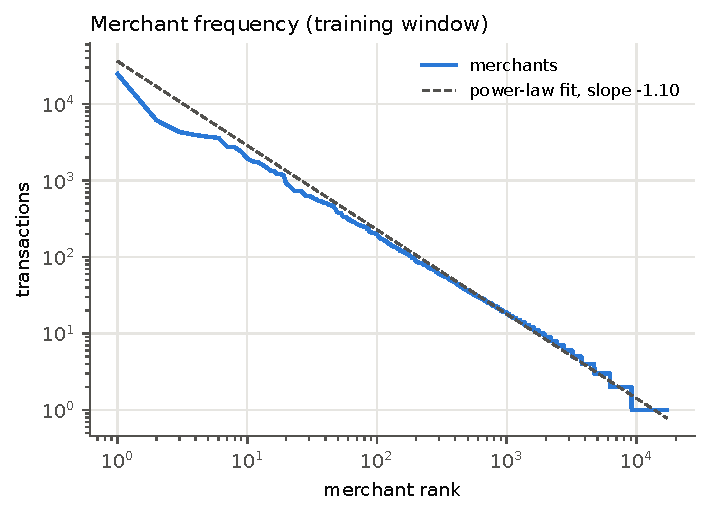
\includegraphics[width=0.48\textwidth]{../results/figures/fig1_zipf.pdf}
\hfill
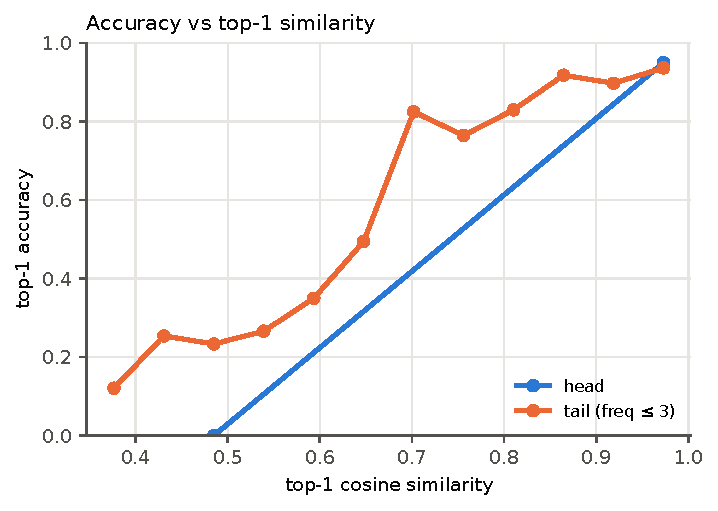
\includegraphics[width=0.48\textwidth]{../results/figures/fig3_acc_vs_sim.pdf}
\caption{Left: merchant rank-frequency in the training window, log-log, with a fitted slope of
$-1.10$; 47\% of merchants occur exactly once. Right: top-1 accuracy against top-1 cosine
similarity, head and tail. The two panels together are the argument for the routed design: the tail
is large, and the encoder knows when it is lost.}
\label{fig:tail}
\end{figure}

Merchant frequency follows the expected power law (Figure~\ref{fig:tail}, left). The interesting
result is what that does to accuracy.

\begin{table}[t]
\centering
\caption{kNN accuracy by training frequency (MiniLM-L6-v2, full DC test set). The cliff is at zero: a merchant seen once is classified as well as a merchant seen a thousand times.}
\label{tab:accfreq}
\begin{tabular}{lrrc}
\toprule
Training frequency & Test txns & Top-1 accuracy & 95\% CI\\
\midrule
0 (unseen) & 14,983 & 0.599 & [0.591, 0.607] \\
1 & 2,168 & 0.960 & [0.951, 0.968] \\
2-5 & 4,793 & 0.950 & [0.944, 0.956] \\
6-20 & 13,594 & 0.984 & [0.981, 0.986] \\
21-100 & 9,228 & 0.970 & [0.966, 0.973] \\
100+ & 38,349 & 0.931 & [0.928, 0.933] \\
\bottomrule
\end{tabular}
\end{table}


Table~\ref{tab:accfreq} breaks kNN accuracy down by how often the test merchant appeared during
training. Accuracy is flat and high, between 0.93 and 0.98, for every bin with at least one prior
observation, including the singleton bin. It collapses to 0.599 for merchants with zero prior
observations. In other words, the ``long tail problem'' in this domain is not a gradient; it is a
membership test. Once a merchant string is in the index, one occurrence is as good as a thousand,
because the match is essentially exact. The gap between 0.96 at frequency one and 0.60 at frequency
zero is the entire problem.

\paragraph{The generator confirms the mechanism.} Sweeping the Zipf exponent from 0.8 to 1.5 changes
the tail's share of traffic from 60\% to 28\% but moves tail accuracy only from 0.904 to 0.939.
Sweeping the share of brands that appear only after the split date has a far larger effect
(Table~\ref{tab:novelshare}): overall accuracy falls from 0.960 to 0.669 as novel brands go from 0\%
to 30\%, and accuracy on genuinely unseen entities sits near 0.5 no matter which dial is turned.
Skew is not what hurts; novelty is.

\begin{table}[t]
\centering
\caption{Generator sweep over the share of brands that appear only after the split date, with the Zipf exponent held at 1.1 (five seeds). Accuracy on genuinely unseen entities is pinned near 0.5 regardless of the dial; only their share of traffic changes.}
\label{tab:novelshare}
\begin{tabular}{rrrrrr}
\toprule
Novel brand share & Unseen txns & Overall & Tail & Unseen entities & Seen entities\\
\midrule
0.00 & 1.1\% & 0.960 & 0.912 & 0.474 & 0.966 \\
0.05 & 12.1\% & 0.918 & 0.841 & 0.540 & 0.967 \\
0.10 & 22.1\% & 0.867 & 0.765 & 0.513 & 0.966 \\
0.20 & 39.7\% & 0.770 & 0.652 & 0.473 & 0.968 \\
0.30 & 58.8\% & 0.669 & 0.570 & 0.459 & 0.968 \\
\bottomrule
\end{tabular}
\end{table}


\subsection{The gate}
\label{sec:gate}

For routing to be economical, the encoder must know when it is lost. It does. Top-1 cosine
similarity separates the two regimes cleanly (Figure~\ref{fig:tail}, right): below the 0.65
threshold, accuracy is 0.325; at or above it, 0.934. Only 7.9\% of test transactions fall below the
threshold, and 98.4\% of those are tail merchants. A threshold on a single scalar is therefore enough
to buy most of what a learned gate could offer, which is why we keep it.

\section{Main comparison}
\label{sec:main}

\begin{table}[t]
\centering
\caption{Main comparison on the 3,000-merchant fallback evaluation set (2,500 tail, 500 head), macro-F1, five seeds. Cost is US dollars per 1,000 transactions at list prices; fallback is the share of transactions sent to the LLM.}
\label{tab:main}
\begin{tabular}{lrrrrr}
\toprule
Method & Overall & Head & Tail & USD/1k & Fallback\\
\midrule
\multicolumn{6}{l}{\textit{Retrieval only}} \\
kNN, MiniLM-L6-v2 & 0.807 & 0.952 & 0.607 & -- & -- \\
kNN, bge-small-en-v1.5 & 0.820 & 0.952 & 0.637 & -- & -- \\
kNN, text-embedding-3-small & 0.822 & 0.952 & 0.643 & -- & -- \\
Logistic regression on MiniLM embeddings & 0.619 & 0.749 & 0.399 & -- & -- \\
\multicolumn{6}{l}{\textit{LLM only, every merchant}} \\
gpt-5-nano, no web & 0.444 & 0.461 & 0.354 & $<$0.01 & 100.0\% \\
gpt-5-nano, web evidence & 0.542 & 0.541 & 0.485 & 1.59 & 100.0\% \\
gpt-5-mini, no web & 0.507 & 0.518 & 0.424 & 0.03 & 100.0\% \\
gpt-5-mini, web evidence & 0.588 & 0.576 & 0.543 & 1.63 & 100.0\% \\
\multicolumn{6}{l}{\textit{Routed: kNN, similarity gate at 0.65, LLM with web evidence}} \\
Routed, gpt-5-nano & 0.799 & 0.952 & 0.670 & 0.53 & 10.4\% \\
\textbf{Routed, gpt-5-mini} & 0.861 & 0.952 & 0.733 & 0.54 & 10.4\% \\
\bottomrule
\end{tabular}
\vspace{2pt}
\footnotesize Open-weight models are evaluated on a 300-merchant tail subset and appear in Table~\ref{tab:ablation}. The routed system is the only configuration that keeps head accuracy while moving the tail.
\end{table}


Table~\ref{tab:main} compares retrieval, language-model-only, and routed systems on the 3{,}000
merchant evaluation set.

Three things stand out. First, \textbf{the language model alone is a bad categorizer}: gpt-5-mini
with web evidence reaches 0.588 macro-F1 against 0.807 for a 22M-parameter encoder doing
nearest-neighbor lookup, and 0.507 without evidence. Whatever the fallback is for, it is not
replacing retrieval. Second, \textbf{routing captures the complement}: the routed system keeps
retrieval's head F1 exactly (0.952, because almost no head merchant falls below the gate) and lifts
tail F1 from 0.607 to 0.733, a 12.6 point gain, for 10.4\% of transactions routed. Third,
\textbf{model size matters less than evidence access, but it does matter at the margin}: routing to
gpt-5-nano yields 0.670 tail F1 against 0.733 for gpt-5-mini at essentially identical cost, because
cost here is dominated by the search call, not by tokens.

\begin{figure}[t]
\centering
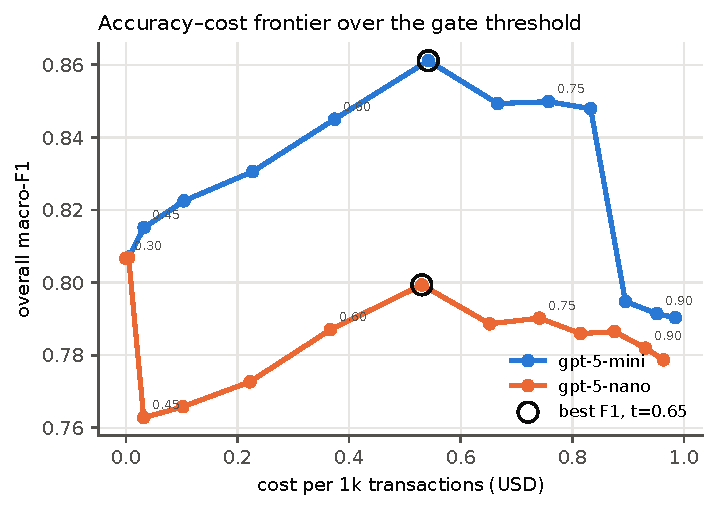
\includegraphics[width=0.72\textwidth]{../results/figures/fig4_acc_cost_frontier.pdf}
\caption{Accuracy-cost frontier over gate thresholds from 0.30 to 0.95. Cost is dollars per thousand
transactions; the marked point is the best threshold for each model. Routing more traffic past 0.65
buys nothing: the transactions it adds are ones retrieval was already getting right.}
\label{fig:frontier}
\end{figure}

Figure~\ref{fig:frontier} sweeps the gate threshold. The frontier is not monotone. Macro-F1 peaks at
$t=0.65$ (0.861) and \emph{falls} to 0.848 at $t=0.70$ and 0.790 at $t=0.90$, while cost rises to
\$0.95 per thousand. Sending more work to the model makes the system worse, because above the
threshold the model is less accurate than the retrieval it overrides. The gate is not a cost dial
with an accuracy penalty; it has a genuine optimum, and it is cheap.

\section{Is it the evidence or the model?}
\label{sec:ablation}

The central claim of any retrieval-augmented result is that the retrieved evidence, not the model,
is responsible. We test it directly: same merchants, same taxonomy, same prompt template, with the
web results block present or absent.

\begin{table}[t]
\centering
\caption{The critical ablation: identical prompts, merchants and taxonomy, with and without web search evidence. Paired bootstrap over merchants; every interval excludes zero.}
\label{tab:ablation}
\small
\begin{tabular}{lrrrrc}
\toprule
Fallback model & Merchants & No web & With web & Difference & 95\% CI\\
\midrule
gpt-5-nano & 2,500 & 0.362 & 0.537 & \textbf{+0.175} & [+0.155, +0.195] \\
DiffusionGemma 26B-A4B & 300 & 0.490 & 0.630 & \textbf{+0.140} & [+0.083, +0.197] \\
gpt-5-mini & 2,500 & 0.501 & 0.624 & \textbf{+0.124} & [+0.106, +0.141] \\
Muse Glimmer 30B & 298 & 0.503 & 0.607 & \textbf{+0.104} & [+0.050, +0.158] \\
Nemotron 3 Super 120B-A12B & 319 & 0.511 & 0.577 & \textbf{+0.066} & [+0.016, +0.116] \\
\bottomrule
\end{tabular}
\vspace{4pt}
\begin{minipage}{0.86\textwidth}\footnotesize The three open-weight models run on NVIDIA's free NIM endpoint and are evaluated on the shared 300-merchant tail subset, which is why their intervals are wider.\end{minipage}
\end{table}


The effect is unambiguous (Table~\ref{tab:ablation}). Across five models spanning two orders of
magnitude in size, and including three open-weight models we did not select for performance, web
evidence adds between 6.6 and 17.5 accuracy points, and every paired-bootstrap interval over
merchants excludes zero. The gain is \emph{larger} for the smaller commercial model ($+0.175$ for
gpt-5-nano against $+0.124$ for gpt-5-mini), which is what one expects if the evidence is supplying
facts the model lacks rather than reasoning it lacks.

This also settles a cheaper hypothesis: that a large model already knows these merchants from
pretraining. It does not. Without evidence, gpt-5-mini scores 0.501 on tail merchants. These are
small, local, or recently founded businesses, exactly the entities least likely to be memorized.

\subsection{Cold start across institutions}
\label{sec:coldstart}

\begin{table}[t]
\centering
\caption{Cross-dataset cold start: 800 Oklahoma merchants that never appear in the DC training index, classified with the DC index and taxonomy.}
\label{tab:coldstart}
\begin{tabular}{lr}
\toprule
Method & Macro-F1\\
\midrule
kNN on the DC index & 0.392 \\
gpt-5-nano, no web & 0.321 \\
gpt-5-nano, web evidence & 0.459 \\
gpt-5-mini, no web & 0.503 \\
gpt-5-mini, web evidence & 0.576 \\
\bottomrule
\end{tabular}
\end{table}


Table~\ref{tab:coldstart} repeats the comparison on 800 Oklahoma merchants absent from the DC index,
the situation a new customer or a new geography presents. Retrieval scores 0.392, essentially the
guessing regime from Section~\ref{sec:tail}. The web-augmented fallback scores 0.576. Note that here
the no-evidence model (0.503) also beats retrieval, because retrieval has nothing to work with; the
evidence still adds 7.3 points on top.

\subsection{Agentic search and prompt sensitivity}
\label{sec:agentic}

\begin{table}[t]
\centering
\caption{Letting the model run its own searches instead of reading five fixed snippets (gpt-5-mini, the shared 300-merchant tail subset).}
\label{tab:agentic}
\begin{tabular}{lrrr}
\toprule
Evidence strategy & Accuracy & Searches/merchant & USD/1k\\
\midrule
No web evidence & 0.513 & -- & -- \\
Fixed web snippets (this paper) & 0.613 & 1.00 & 1.63 \\
Agent-issued searches & 0.620 & 1.64 & 21.16 \\
\bottomrule
\end{tabular}
\vspace{2pt}
\footnotesize Prompt sensitivity on the same subset, two independently written prompt templates: gpt-5-nano no web 1.7 pts, gpt-5-nano with web 2.7 pts, gpt-5-mini no web 2.3 pts, gpt-5-mini with web 1.3 pts. Prompt wording moves accuracy by a few points; web evidence moves it by ten to seventeen.
\end{table}


Two robustness checks (Table~\ref{tab:agentic}). Letting the model issue its own searches through a
built-in web-search tool, rather than reading five snippets we fetched, scores 0.620 against 0.613,
a difference of two merchants out of 300, at 13$\times$ the cost (\$21.16 against \$1.63 per
thousand). For this task the expensive agentic loop is not worth its price; one well-formed query
with the merchant string is what matters. Separately, rewriting both prompts from scratch moves
accuracy by 1.3 to 2.7 points, against the 10 to 17 points attributable to evidence, so the headline
effect is not a prompt artifact.

\section{Streaming write-back}
\label{sec:stream}

If the fallback resolves a merchant today, the system should not pay for it again tomorrow. We
replay 70{,}333 test transactions in arrival order through 141 windows of 500, with five write-back
policies: never write; always write the resolved label; or write only when the model's self-reported
confidence exceeds a threshold.

\begin{table}[t]
\centering
\caption{Streaming write-back over 70,333 test transactions in arrival order (141 windows, five seeds). Writing every resolved merchant back into the index halves the fallback bill and costs 0.3 points of macro-F1, but nearly half of the written labels are wrong.}
\label{tab:writeback}
\begin{tabular}{lrrrrrr}
\toprule
Write-back policy & Fallback & Macro-F1 & Total USD & Writes & Wrong writes & Index size\\
\midrule
never & 2.99\% & 0.909 & 22.62 & 0 & 0.0\% & 14,878 \\
gated@0.8 & 2.99\% & 0.909 & 22.61 & 2 & 0.0\% & 14,880 \\
gated@0.7 & 2.55\% & 0.905 & 19.26 & 180 & 22.8\% & 15,058 \\
gated@0.6 & 2.15\% & 0.905 & 16.24 & 446 & 36.1\% & 15,324 \\
gated@0.5 & 1.74\% & 0.906 & 13.20 & 709 & 40.6\% & 15,587 \\
always & 1.37\% & 0.906 & 10.38 & 948 & 46.8\% & 15,826 \\
\bottomrule
\end{tabular}
\end{table}


\begin{figure}[t]
\centering
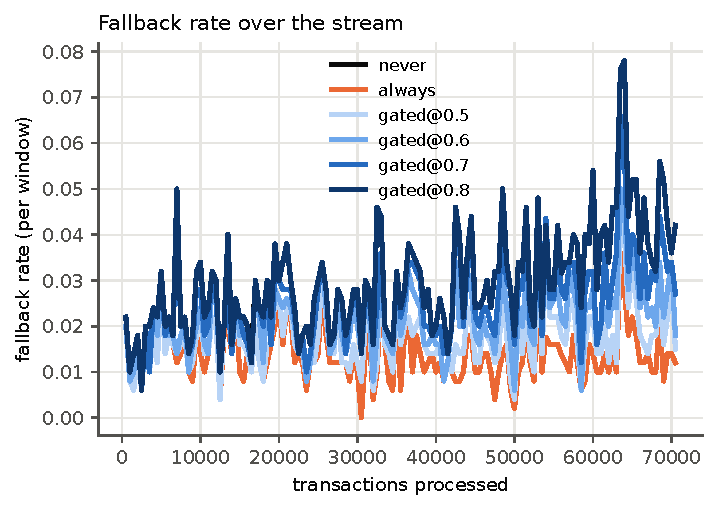
\includegraphics[width=0.48\textwidth]{../results/figures/fig5_fallback_decay.pdf}
\hfill
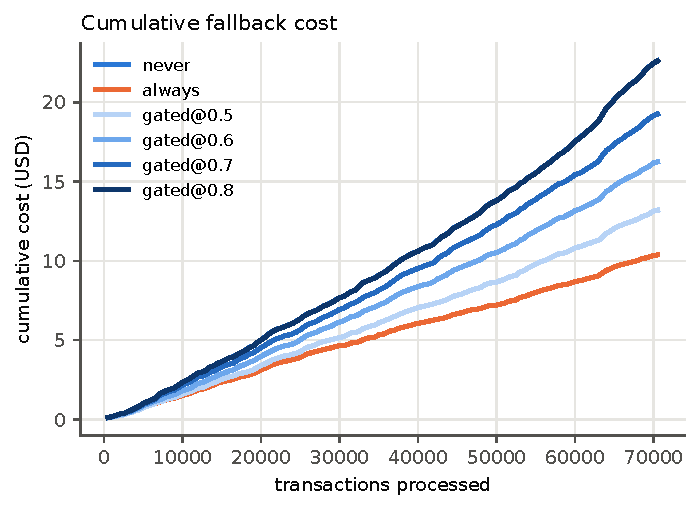
\includegraphics[width=0.48\textwidth]{../results/figures/fig6_cumulative_cost.pdf}
\caption{Left: fallback rate per window under each policy. Right: cumulative spend. Write-back bends
the cost curve early and permanently, because a resolved merchant is answered by retrieval from then
on.}
\label{fig:stream}
\end{figure}

Writing every resolved merchant back halves the bill, from \$22.62 to \$10.38 over the stream, and
cuts the steady-state fallback rate from 2.99\% to 1.37\% (Table~\ref{tab:writeback},
Figure~\ref{fig:stream}), at a cost of 0.3 points of macro-F1. For most deployments that is an easy
trade.

The uncomfortable number is the next column: \textbf{46.8\% of the written labels are wrong}. The
system halves its costs while filling its own index with errors, and the aggregate metric barely
notices, because the merchants being written are rare by construction and their errors are diluted.
Anyone running this in production should measure the write path separately from the serving path;
an aggregate F1 will not reveal the rot.

Confidence gating on the write path does not rescue it. Raising the write threshold monotonically
reduces both the number of writes and their error rate, but it also removes the savings: at $t=0.8$
the policy writes 2 merchants out of 948 candidates and is indistinguishable from never writing.
These models' self-reported confidence is not calibrated finely enough to separate right from wrong
answers at any threshold that preserves the benefit \citep{guo2017calibration}. A verification step
with independent evidence, rather than self-reported confidence, is the obvious next design.

\section{Which encoder?}
\label{sec:backbones}

\begin{table}[t]
\centering
\caption{Embedding backbones under the same index, gate and taxonomy, full DC test set, five seeds. Twenty-three times the embedding latency buys one point of tail macro-F1.}
\label{tab:backbones}
\begin{tabular}{lrrrrrr}
\toprule
Backbone & Dim & ms/merchant & Overall & Head & Tail & Tail acc.\\
\midrule
MiniLM-L6-v2 & 384 & 0.53 & 0.846 & 0.932 & 0.633 & 0.689 \\
bge-small-en-v1.5 & 384 & 0.91 & 0.851 & 0.932 & 0.634 & 0.695 \\
mpnet-base-v2 & 768 & 2.57 & 0.851 & 0.932 & 0.639 & 0.692 \\
FinBERT & 768 & 2.08 & 0.817 & 0.932 & 0.537 & 0.593 \\
text-embedding-3-small & 1536 & 11.96 & 0.852 & 0.932 & 0.644 & 0.715 \\
\bottomrule
\end{tabular}
\end{table}


Table~\ref{tab:backbones} holds the index, gate, and taxonomy fixed and varies only the encoder, on
the full test set. The spread is small and the ordering is boring: a commercial 1536-dimensional
embedding is 1.1 points of tail macro-F1 better than a 384-dimensional CPU model at 23$\times$ the
encoding latency and a per-merchant API cost. Domain pretraining actively hurts: FinBERT, trained on
financial text, is 9.6 points of tail F1 worse than general-purpose MiniLM, presumably because
merchant descriptors are names, not prose about finance. Given Section~\ref{sec:tail}, none of this
is surprising: no encoder can embed a merchant it has never seen into the right neighborhood, so
encoder quality cannot address the dominant error mode.

\section{What is actually left}
\label{sec:failures}

We sampled 200 residual errors of the routed system on tail merchants and labeled each by hand.

\begin{table}[t]
\centering
\caption{Manual taxonomy of 200 residual tail errors made by the routed system with web evidence. Two thirds are annotation or taxonomy artifacts rather than model failures.}
\label{tab:failures}
\begin{tabular}{lrrl}
\toprule
Failure class & Count & Share & Example merchant\\
\midrule
taxonomy mismatch & 101 & 50.5\% & \texttt{WOMEN IN HOUSING \& FIN} \\
label noise & 34 & 17.0\% & \texttt{MAC-ISA} \\
LLM reasoning error & 16 & 8.0\% & \texttt{BIO COMPANY INC} \\
no web presence & 15 & 7.5\% & \texttt{AUTOAUTH SERVICE} \\
web search failure & 15 & 7.5\% & \texttt{GESSCREATIONS} \\
ambiguous merchant & 13 & 6.5\% & \texttt{NATIONAL SEATING} \\
normalization failure & 6 & 3.0\% & \texttt{COURSRA2A12B1FKC1KV9Q} \\
\bottomrule
\end{tabular}
\end{table}


Table~\ref{tab:failures} reorders the priorities. Half of the ``errors'' are taxonomy mismatches: the
merchant is correctly identified and the predicted category is defensible, but the
merchant-category-code label assigns it elsewhere. A women's housing-finance association is coded by
the acquirer as a membership organization and predicted as professional services; both are right
under different readings of a 15-way taxonomy. A further 17\% are outright label noise, consistent
with the independent 300-row audit in Section~\ref{sec:data}. Together, two thirds of what the metric
counts as failure is annotation artifact.

The genuinely addressable slice is smaller than the headline gap suggests: 8\% model reasoning
errors, 7.5\% merchants with no usable web presence, 7.5\% search failures where results existed but
missed, 6.5\% genuinely ambiguous merchants, and 3\% normalization failures where the descriptor was
mangled beyond recovery (for example a truncated course-payment reference). Only about a fifth of the
remaining error is attackable by better search or a better model; the rest requires changing the
label definition, which is a product decision rather than a modeling one.

\section{Limitations}

\textbf{Domain.} Both datasets are US government purchase-card programs. The merchant mix skews to
office supply, industrial, and travel spending, and away from consumer categories such as groceries
and restaurants. The mechanism we measure, that unseen merchants collapse and web evidence restores
them, should transfer; the exact numbers should not be assumed to.

\textbf{Labels.} Merchant category codes are assigned by acquirers for interchange purposes, not for
analytics. They are noisy at 4.4\% and ambiguous at up to 19.7\% (Section~\ref{sec:data}), and
Section~\ref{sec:failures} shows this dominates the residual. Any comparison of systems above roughly
0.85 macro-F1 on this data is measuring annotation as much as capability.

\textbf{Web drift.} Search results were collected in September 2026 and frozen. The same queries
tomorrow return different pages, so the absolute fallback numbers are a snapshot. This is an inherent
property of web-augmented systems and an argument for caching evidence alongside predictions, which
is also what makes this paper reproducible.

\textbf{Open-weight coverage.} The three open-weight models were evaluated on a 300-merchant tail
subset because the free endpoint serializes requests; their intervals are wide and they are not
directly comparable to the commercial models' full-set numbers.

\textbf{Single fallback design.} We did not test multi-step verification, ensembling several models,
or feeding the retrieved neighbors to the model as additional context. The write-back result in
Section~\ref{sec:stream} suggests verification is the highest-value missing piece.

\section{Conclusion}

Embedding retrieval for transaction categorization fails in a specific, measurable way: it is
near-perfect on merchants it has seen even once, and it collapses on merchants it has never seen,
which are a fifth of real traffic under a temporal split. Because the failure is a missing-knowledge
problem rather than a sample-size problem, the effective fix is to give a language model external
evidence about the unseen merchant and to spend that model only where retrieval reports low
confidence. That routed design lifts tail macro-F1 by 12.6 points for \$0.54 per thousand
transactions, and the gain survives ablation across five models: it is the web evidence doing the
work, not the language model. Two cautions carry beyond this dataset. Writing model answers back into
the index halves cost and quietly fills the index with errors at a 47\% rate, and the accuracy ceiling
is set by the taxonomy and the labels rather than by the models, since two thirds of residual errors
are annotation artifacts.

\section*{Reproducibility}

The repository contains the pipeline, the frozen prompts with their hashes, pinned model identifiers,
the committed API caches (17{,}764 language model calls, 3{,}869 searches, and float16 embedding
caches for five encoders), and the taxonomy and audit files.
\texttt{python reproduce.py --config configs/dc.yaml} regenerates every table and figure from those
caches with no network access and verifies each regenerated table against the committed copy;
a run manifest records package versions, prompt hashes, index parameters, git commit, and host. A
Dockerfile builds the same environment. Table~\ref{tab:spend} reports total spend.

\begin{table}[t]
\centering
\caption{Total API spend for every experiment in this paper. The frozen caches hold 19,265 LLM calls and 4,388 search calls; reproduce.py replays them and issues no requests.}
\label{tab:spend}
\begin{tabular}{lr}
\toprule
Item & USD\\
\midrule
OpenAI chat completions (cache pass, all experiments) & 3.07 \\
OpenAI built-in web search ablation (300 merchants) & 6.38 \\
Firecrawl search (prepaid credits, reference price) & 41.44 \\
NVIDIA NIM open-weight models (free endpoint) & 0.00 \\
\textbf{Total cash spent (OpenAI)} & \textbf{9.45} \\
\bottomrule
\end{tabular}
\end{table}


\bibliographystyle{plainnat}
\bibliography{refs}

\end{document}
